\chapter{Analyse}\label{ch:analyse}



\section{Motor}

\begin{figure}[H]
	\centering
	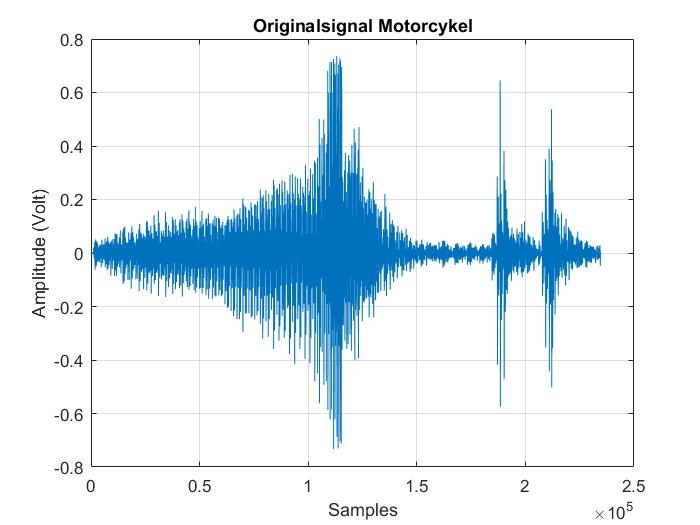
\includegraphics[width=140mm]{figures/Motor/original.jpg}
	\caption{DF140 Det originale signal fra en Motor}
	\label{fig:Motor original}
\end{figure}

\begin{figure}[H]
	\centering
	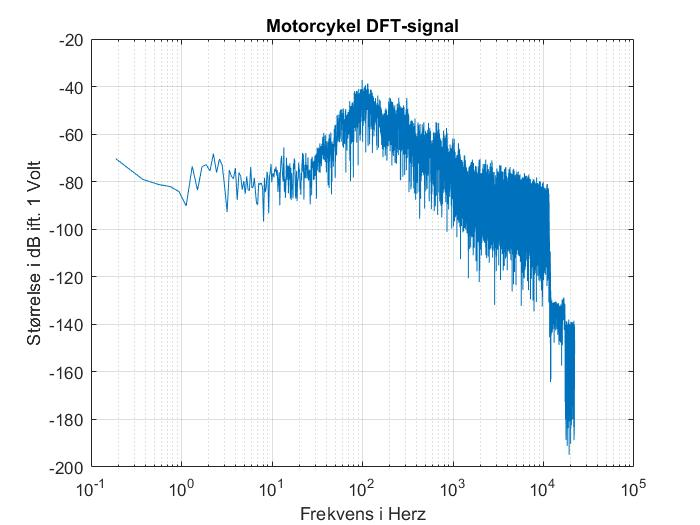
\includegraphics[width=140mm]{figures/Motor/DFT.jpg}
	\caption{DF140 Analyse af et signal fra en Motor}
	\label{fig:Motor DF140}
\end{figure}

\begin{figure}[H]
	\centering
	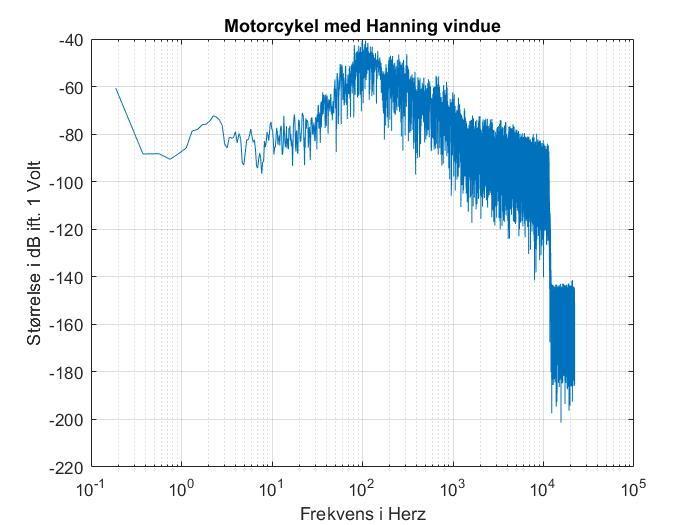
\includegraphics[width=140mm]{figures/Motor/hanning.jpg}
	\caption{DF140 Analyse af et signal fra en Motor med et hanningvindue}
	\label{fig:Motor hanning}
\end{figure}

\begin{figure}[H]
	\centering
	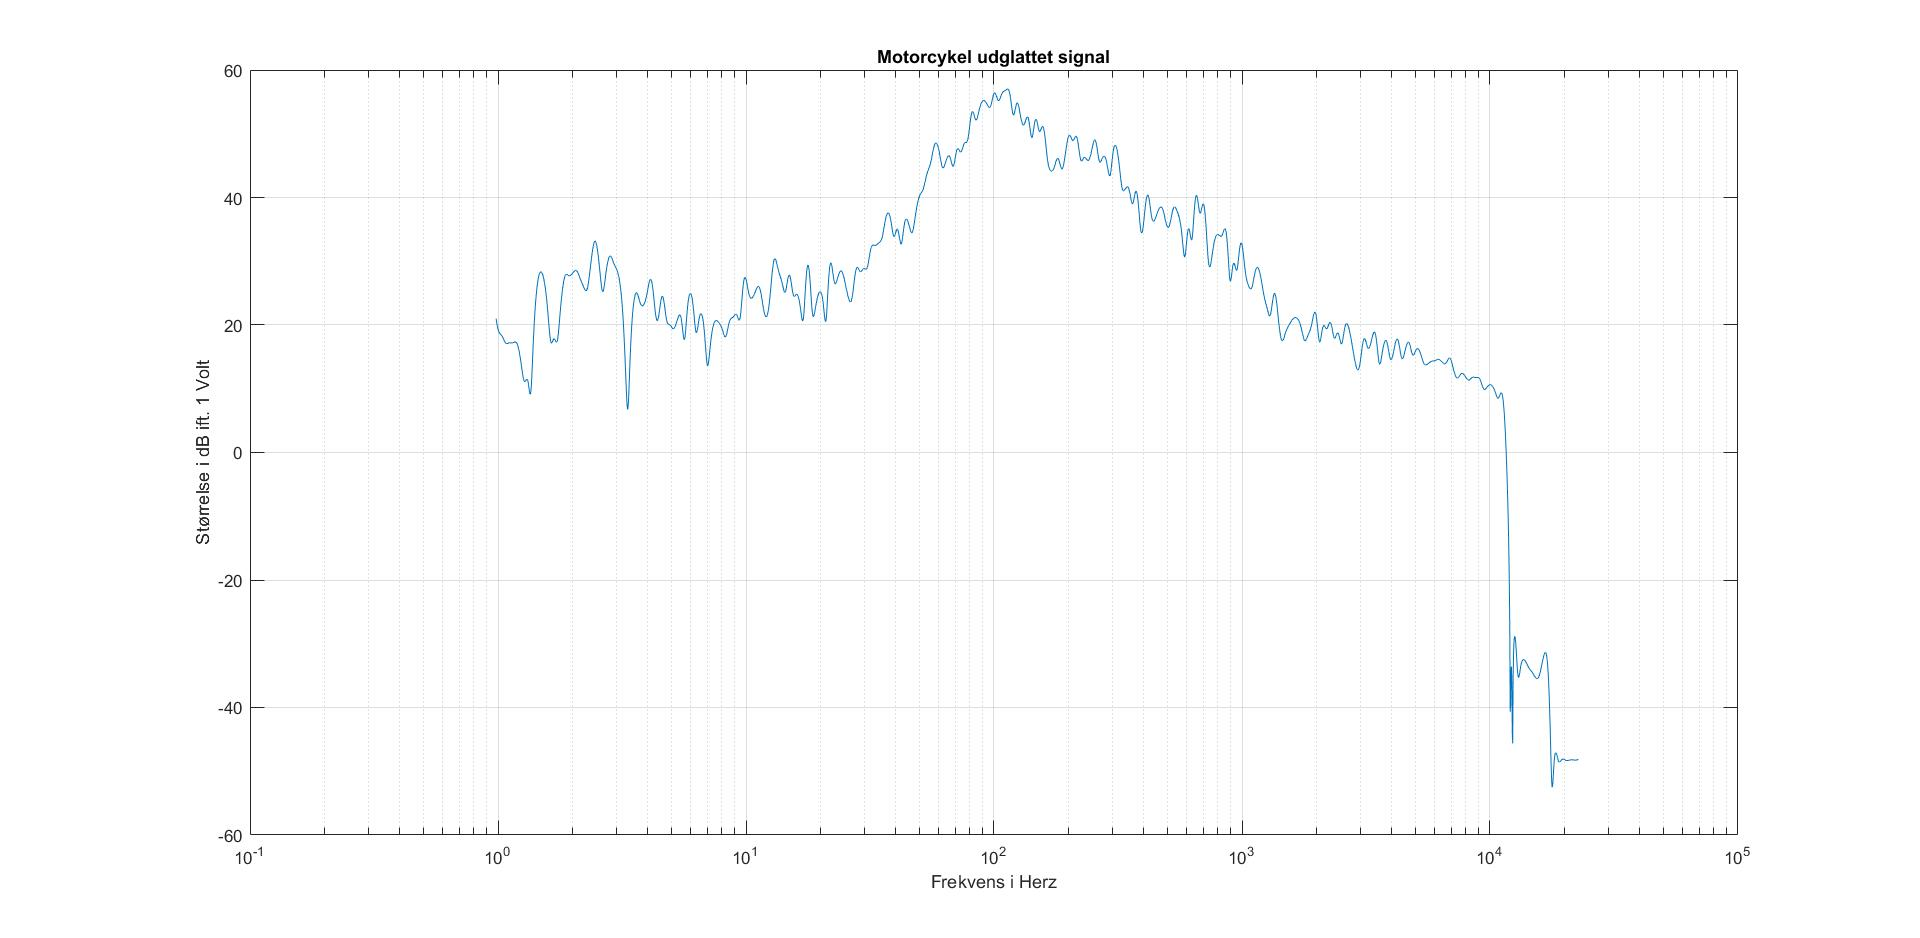
\includegraphics[width=140mm]{figures/Motor/udglattet.jpg}
	\caption{Det udglattede DF140 signal fra en Motor}
	\label{fig:Motor udglattet}
\end{figure}

\section{Klaver}

\begin{figure}[H]
	\centering
	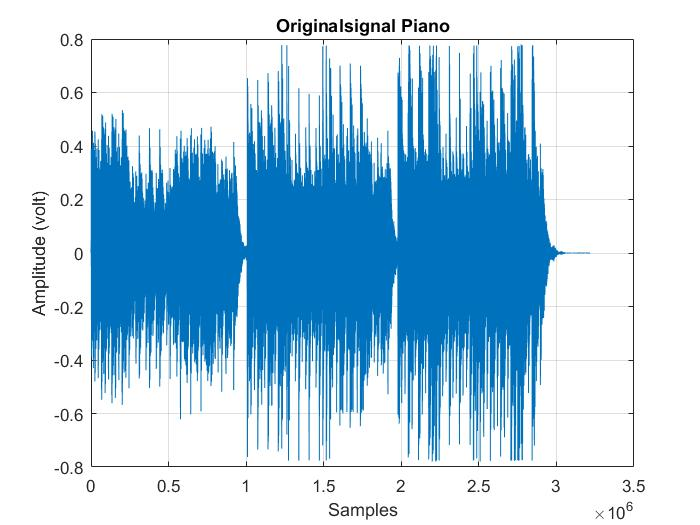
\includegraphics[width=140mm]{figures/Piano/original.jpg}
	\caption{DF140 Det originale signal fra et klaver}
	\label{fig:Klaver original}
\end{figure}

\begin{figure}[H]
	\centering
	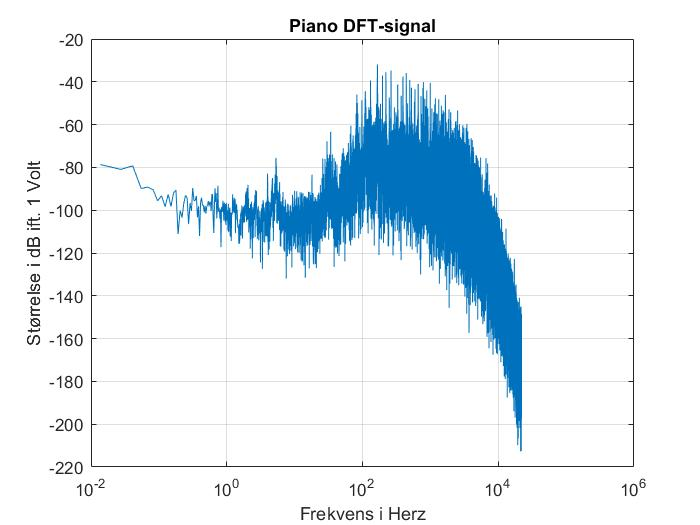
\includegraphics[width=140mm]{figures/Piano/DFT.jpg}
	\caption{DF140 Analyse af et signal fra et Klaver}
	\label{fig:Klaver DF140}
\end{figure}

\begin{figure}[H]
	\centering
	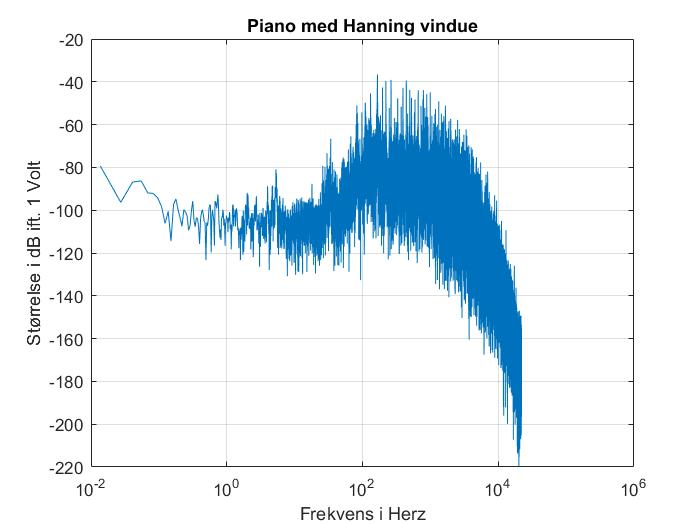
\includegraphics[width=140mm]{figures/Piano/hanning.jpg}
	\caption{DF140 Analyse af et signal fra et klaver med et hanningvindue}
	\label{fig:Klaver hanning}
\end{figure}

\begin{figure}[H]
	\centering
	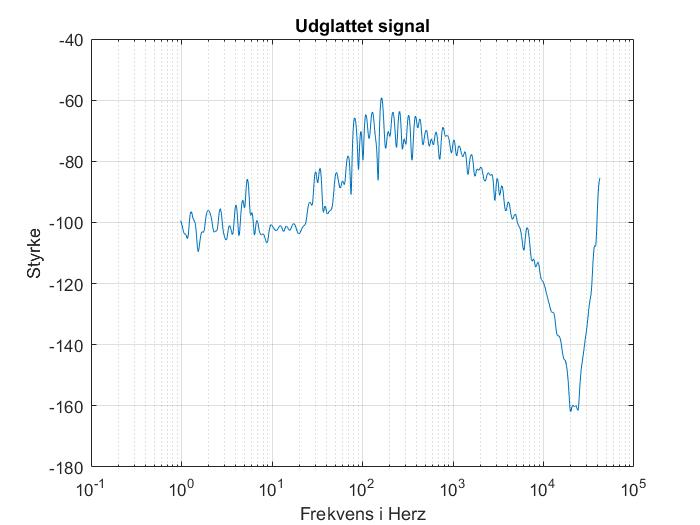
\includegraphics[width=140mm]{figures/Piano/udglattet.jpg}
	\caption{Det udglattede DF140 signal fra et Klaver}
	\label{fig:Klaver udglattet}
\end{figure}
\newpage

\section{Symfoni}

\begin{figure}[H]
	\centering
	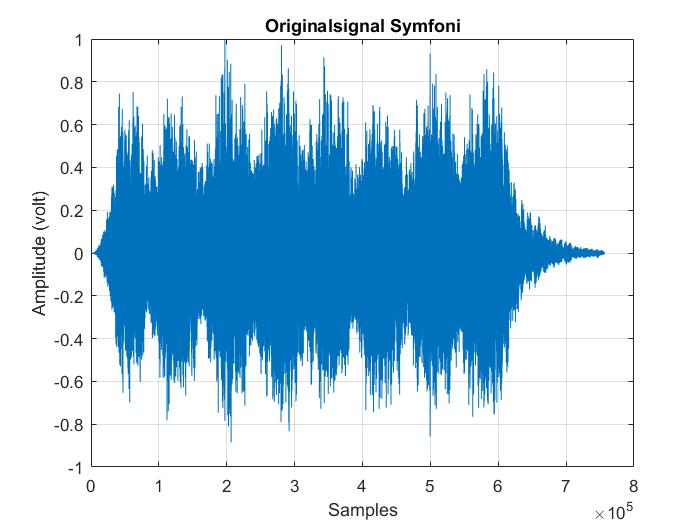
\includegraphics[width=140mm]{figures/Symfoni/original.jpg}
	\caption{DF140 Det originale signal fra en Symfoni}
	\label{fig:Symfoni original}
\end{figure}

\begin{figure}[H]
	\centering
	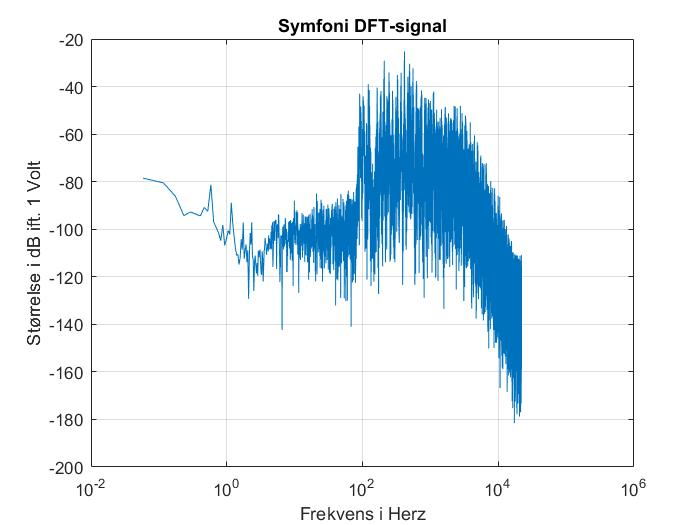
\includegraphics[width=140mm]{figures/Symfoni/DFT.jpg}
	\caption{DF140 Analyse af et signal fra en Symfoni}
	\label{fig:Symfoni DF140}
\end{figure}

\begin{figure}[H]
	\centering
	\includegraphics[width=140mm]{figures/Symfoni/hanning.jpg}
	\caption{DF140 Analyse af et signal fra en Symfoni med et hanningvindue}
	\label{fig:Symfoni hanning}
\end{figure}

\begin{figure}[H]
	\centering
	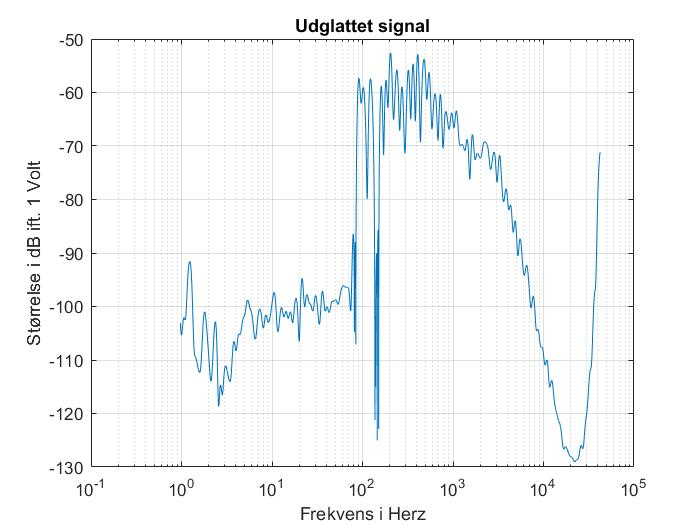
\includegraphics[width=140mm]{figures/Symfoni/udglattet.jpg}
	\caption{Det udglattede DF140 signal fra en Symfoni}
	\label{fig:Symfoni udglattet}
\end{figure}

\section{Bass}

\begin{figure}[H]
	\centering
	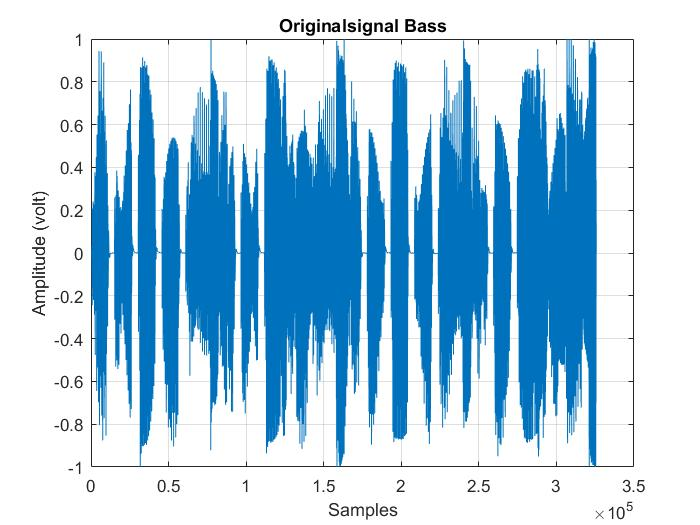
\includegraphics[width=140mm]{figures/Bass/original.jpg}
	\caption{DF140 Det originale signal fra en Bas}
	\label{fig:Bas original}
\end{figure}

\begin{figure}[H]
	\centering
	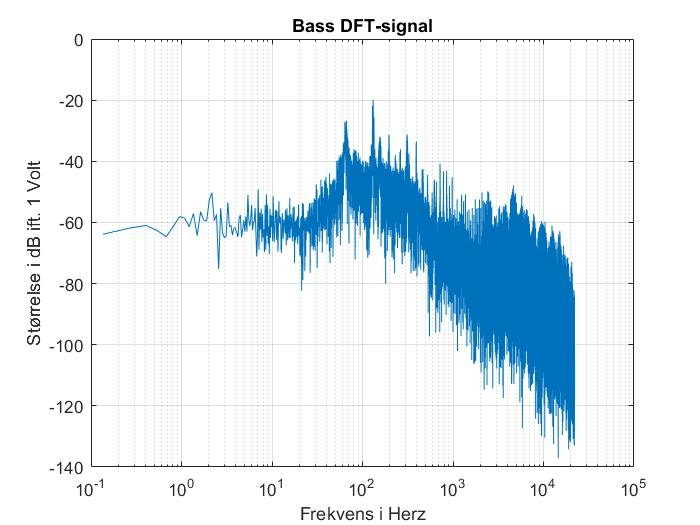
\includegraphics[width=140mm]{figures/Bass/DFT.jpg}
	\caption{DF140 Analyse af et signal fra en Bas}
	\label{fig:Bas DF140}
\end{figure}

\begin{figure}[H]
	\centering
	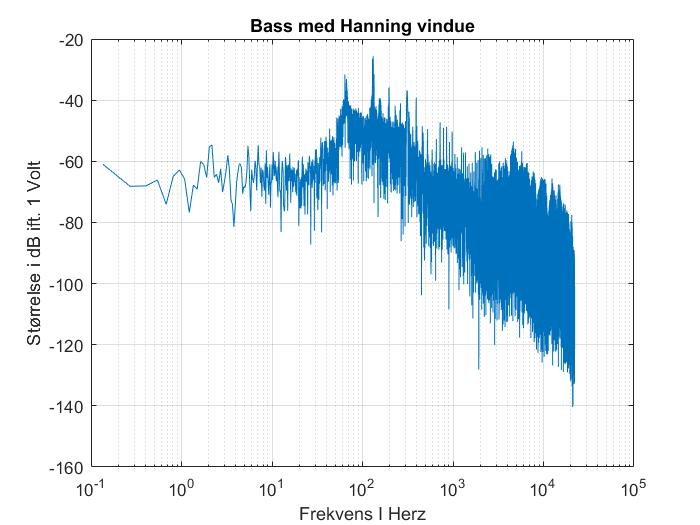
\includegraphics[width=140mm]{figures/Bass/hanning.jpg}
	\caption{DF140 Analyse af et signal fra en Bas med et hanningvindue}
	\label{fig:Bas hanning}
\end{figure}

\begin{figure}[H]
	\centering
	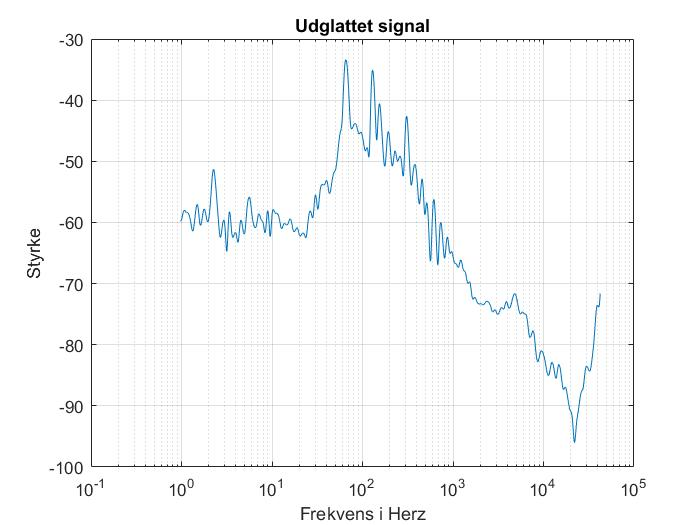
\includegraphics[width=140mm]{figures/Bass/udglattet.jpg}
	\caption{Det udglattede DF140 signal fra en Bas}
	\label{fig:Bas udglattet}
\end{figure}



\section{Vinglas}
\begin{figure}[H]
	\centering
	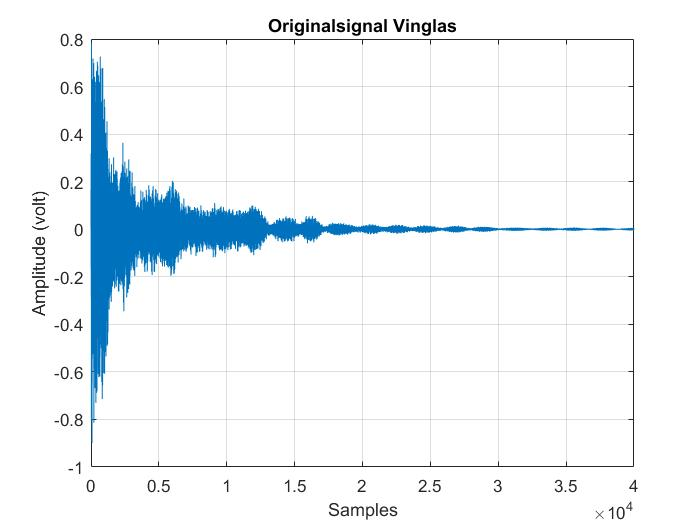
\includegraphics[width=140mm]{figures/Vinglas/original.jpg}
	\caption{DF140 Det originale signal fra et Vinglas}
	\label{fig:Vinglas original}
\end{figure}

\begin{figure}[H]
	\centering
	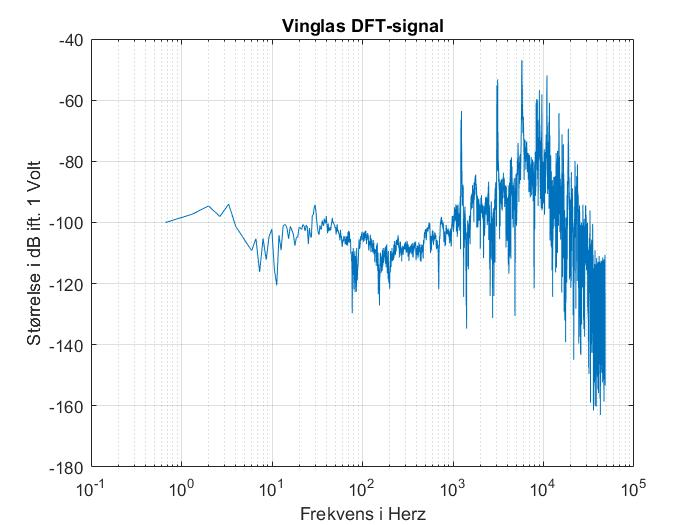
\includegraphics[width=140mm]{figures/Vinglas/DFT.jpg}
	\caption{DF140 Analyse af et signal fra et Vinglas}
	\label{fig:Vinglas DF140}
\end{figure}

\begin{figure}[H]
	\centering
	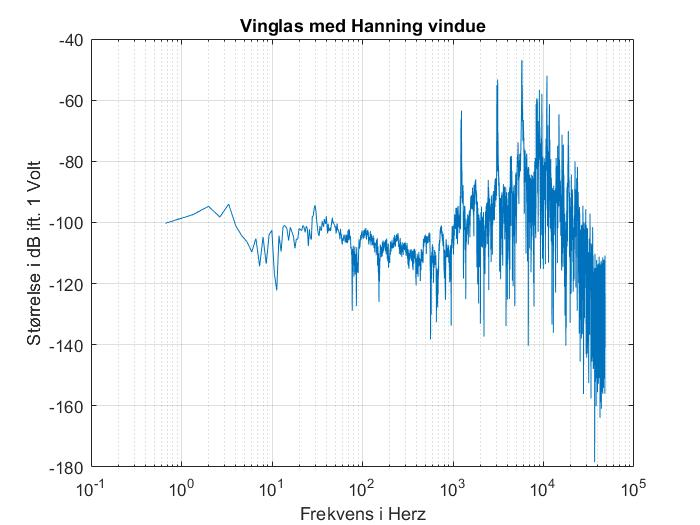
\includegraphics[width=140mm]{figures/Vinglas/hanning.jpg}
	\caption{DF140 Analyse af et signal fra et Vinglas med et hanningvindue}
	\label{fig:Vinglas hanning}
\end{figure}



\section{Vindmølle}
\begin{figure}[H]
	\centering
	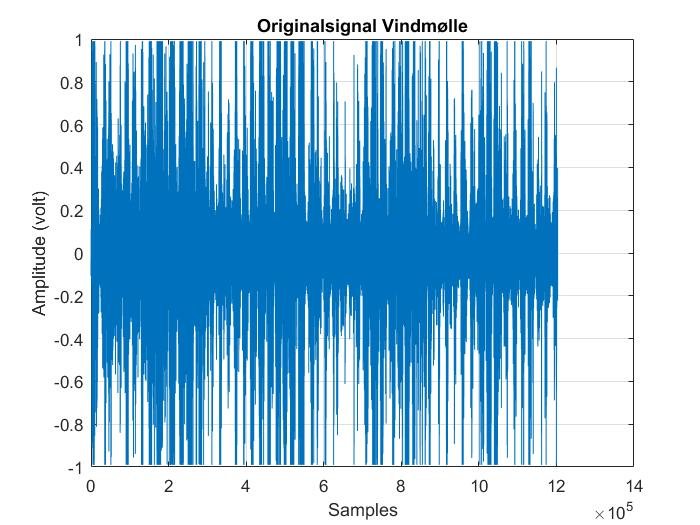
\includegraphics[width=140mm]{figures/Vind/original.jpg}
	\caption{DF140 Det originale signal fra en Vindmølle}
	\label{fig:Vind original}
\end{figure}

\begin{figure}[H]
	\centering
	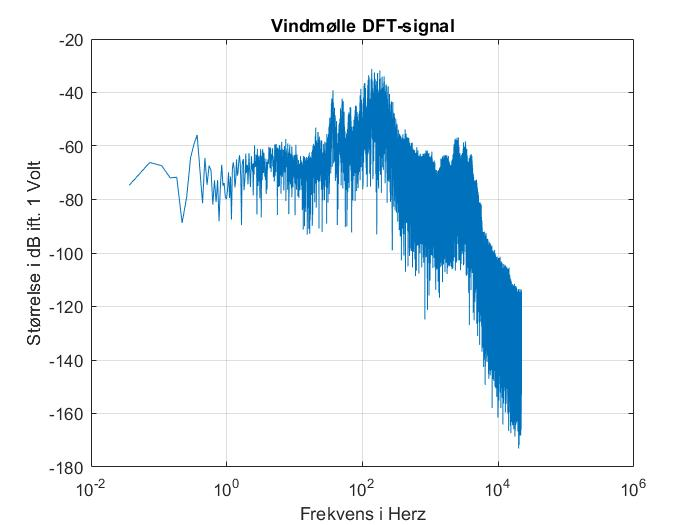
\includegraphics[width=140mm]{figures/Vind/DFT.jpg}
	\caption{DF140 Analyse af et signal fra en Vindmølle}
	\label{fig:Vind DF140}
\end{figure}

\begin{figure}[H]
	\centering
	\includegraphics[width=140mm]{figures/Vind/hanning.jpg}
	\caption{DF140 Analyse af et signal fra en Vindmølle med et hanningvindue}
	\label{fig:Vind hanning}
\end{figure}

\begin{figure}[H]
	\centering
	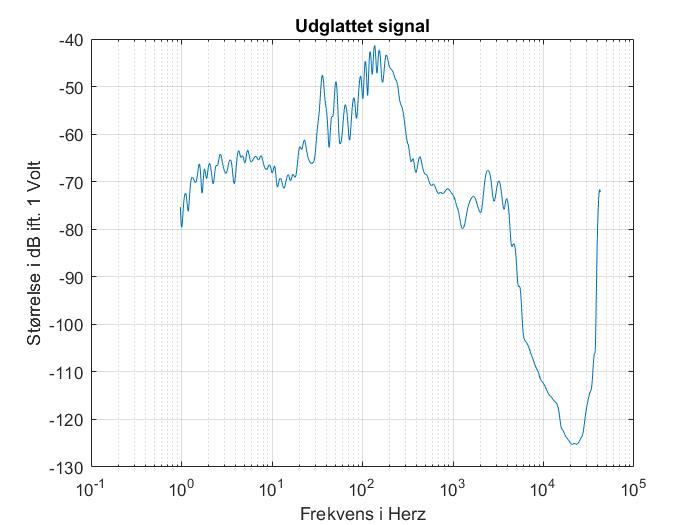
\includegraphics[width=140mm]{figures/Vind/udglattet.jpg}
	\caption{Det udglattede DF140 signal fra en Vindmølle}
	\label{fig:Vind udglattet}
\end{figure}


\section{Musikbox}
\begin{figure}[H]
	\centering
	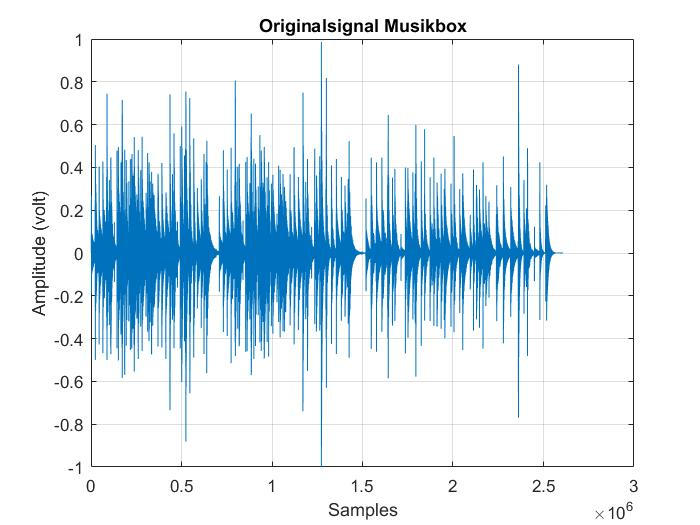
\includegraphics[width=140mm]{figures/Musikbox/original.jpg}
	\caption{DF140 Det originale signal fra en Musikbox}
	\label{fig:Musikbox original}
\end{figure}

\begin{figure}[H]
	\centering
	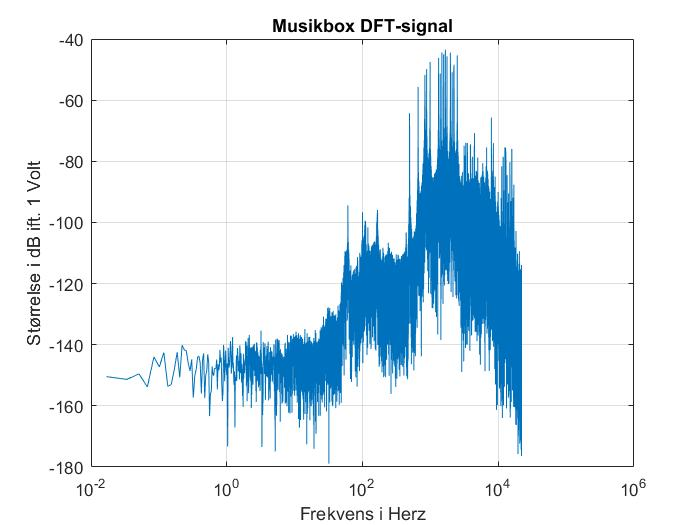
\includegraphics[width=140mm]{figures/Musikbox/DFT.jpg}
	\caption{DF140 Analyse af et signal fra en Musikbox}
	\label{fig:Musikbox DF140}
\end{figure}

\begin{figure}[H]
	\centering
	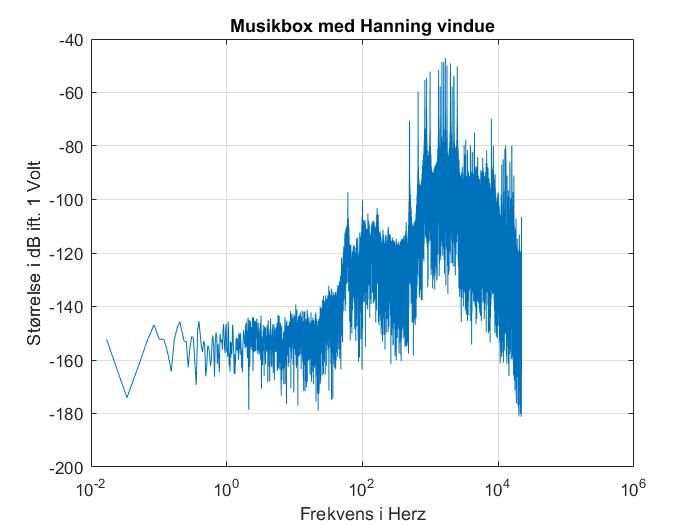
\includegraphics[width=140mm]{figures/Musikbox/hanning.jpg}
	\caption{DF140 Analyse af et signal fra en Musikbox med et hanningvindue}
	\label{fig:Musikbox hanning}
\end{figure}

\begin{figure}[H]
	\centering
	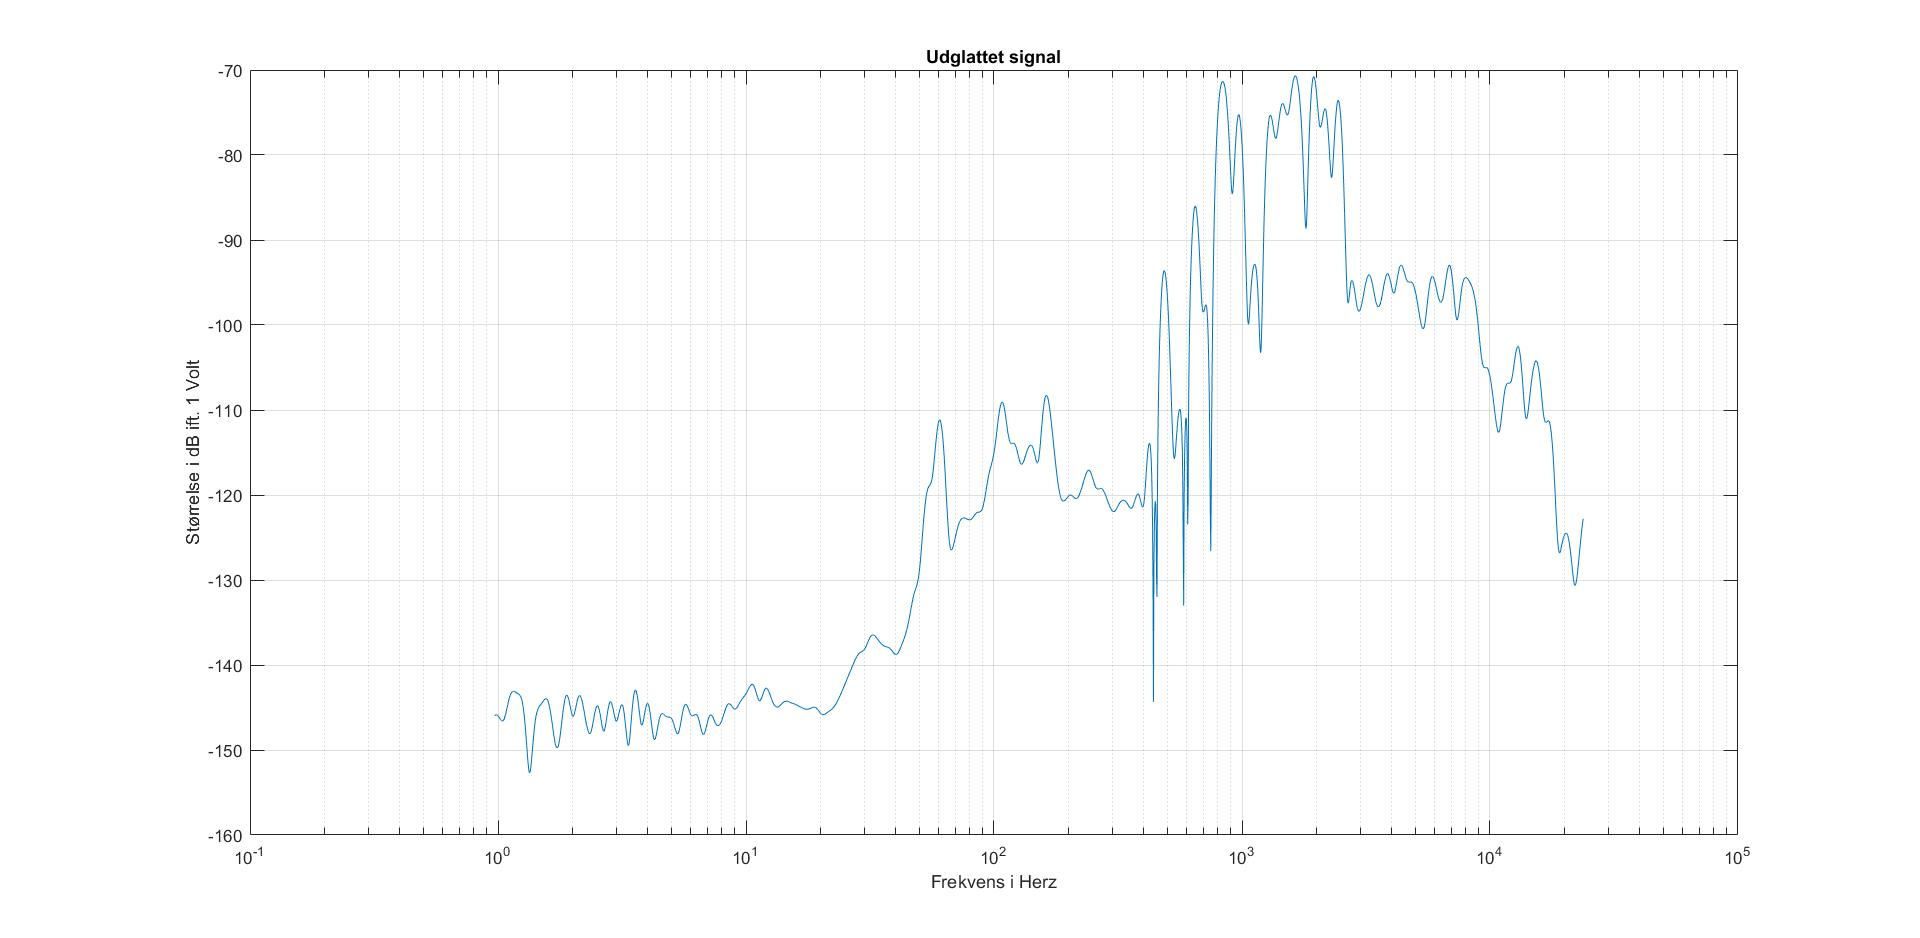
\includegraphics[width=140mm]{figures/Musikbox/udglattet.jpg}
	\caption{Det udglattede DF140 signal fra en Musikbox}
	\label{fig:Musikbox udglattet}
\end{figure}

\section{ECG-signal}
\begin{figure}[H]
	\centering
	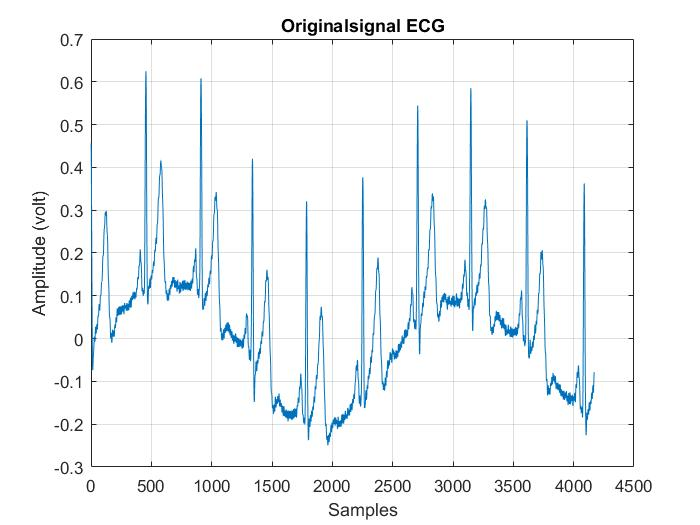
\includegraphics[width=140mm]{figures/ECG/original.jpg}
	\caption{DF140 Det originale ECG-signal}
	\label{fig:ECG original}
\end{figure}

\begin{figure}[H]
	\centering
	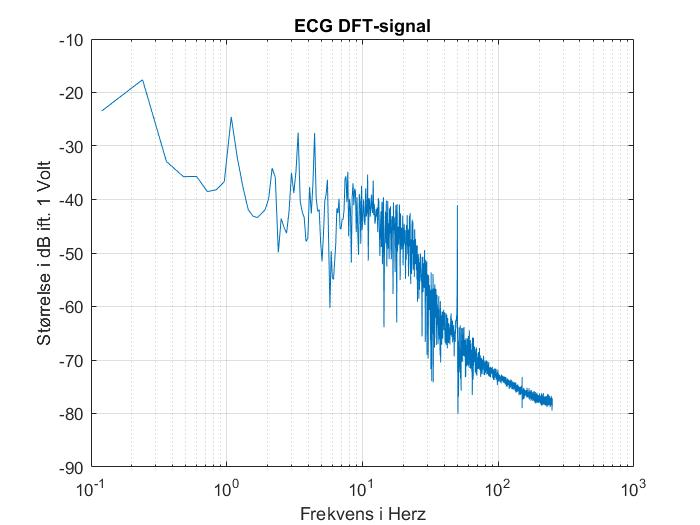
\includegraphics[width=140mm]{figures/ECG/DFT.jpg}
	\caption{DF140 Analyse af et ECG-signal}
	\label{fig:ECG DF140}
\end{figure}

\begin{figure}[H]
	\centering
	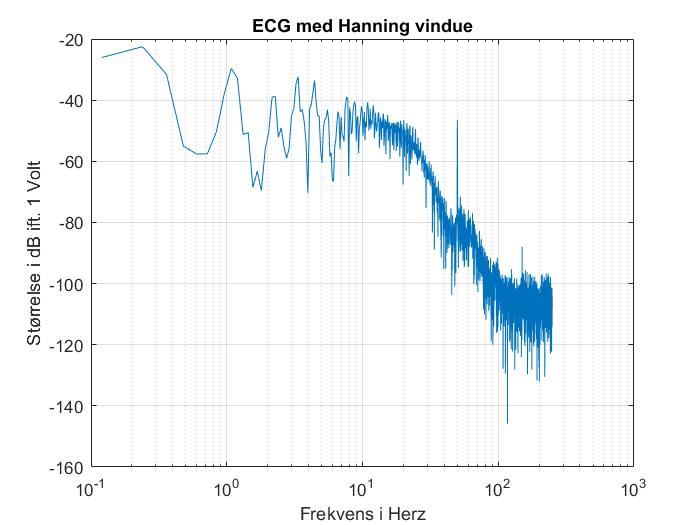
\includegraphics[width=140mm]{figures/ECG/hanning.jpg}
	\caption{DF140 Analyse af et ECG-signal med et hanningvindue}
	\label{fig:ECG hanning}
\end{figure}

\begin{figure}[H]
	\centering
	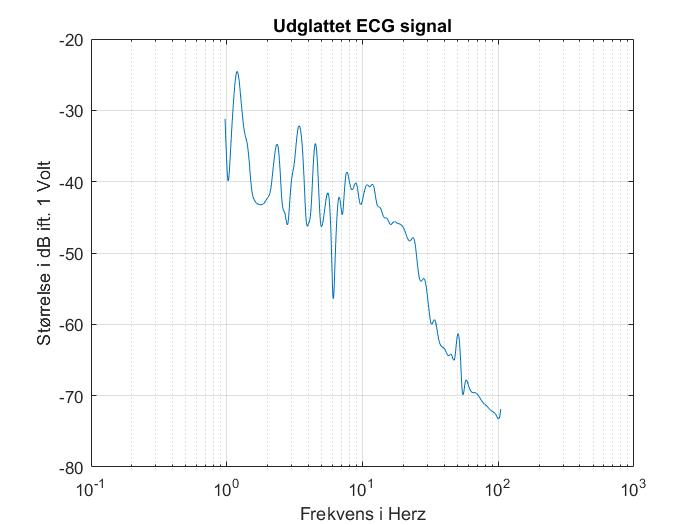
\includegraphics[width=140mm]{figures/ECG/udglattet.jpg}
	\caption{Det udglattede DF140 ECG-signal}
	\label{fig:ECG udglattet}
\end{figure}

